\subsection{AdA shows human-timescale adaptation} \label{sec:results_human_scale_adaptation}

\begin{table}[h!]
  \begin{center}
    \caption{Experimental setup for agent experiments in Section \ref{sec:results_human_scale_adaptation}.}
    \begin{tabular}{c|c|c|c|c|c|c}
    \label{tab:human-timescale-settings}
      \# players & Model parameters & Memory & Task pool & Curriculum & Teacher & Steps\\
      \hline
      1 & 169M TXL / 353M total & 1800 & 25B & PLR \ref{tab:plr_hyperparameters} & \ref{tab:single-agent-teacher} & 100B \\
      2 & 265M TXL / 533M total & 1800 & see App.~\ref{app:multi_agent_training} & PLR \ref{tab:plr_hyperparameters} & \ref{tab:multi-agent-teacher} & 70B \\
    \end{tabular}
  \end{center}
\end{table}

\paragraph{Single-agent.}

In Figure~\ref{fig:single_agent_percentiles} we show the performance of AdA when trained in the single-agent setting described in Table \ref{tab:human-timescale-settings}. Examine first AdA's zero-shot performance ($k=1$, red line). This matches the performance of a baseline agent, trained only in a regime where each episode consists of a single trial. In other words, AdA does not suffer any degradation in zero-shot performance, despite being trained on a distribution over number of trials $k \in \{1, 2, \dots 6\}$. Now turn your attention to AdA's few-shot performance ($k \in \{2, 3, 5, 8, 13\}$, orange to purple lines). Given more trials, AdA improves its performance on over $80\%$ of the task set, clearly adapting at test time. The improvements are particularly strong when comparing zero-shot performance to the two trial setting, but AdA keeps on improving when given more trials. 

\begin{figure}[t]
    \centering
    \begin{subfigure}[b]{0.47\textwidth}
        \centering
        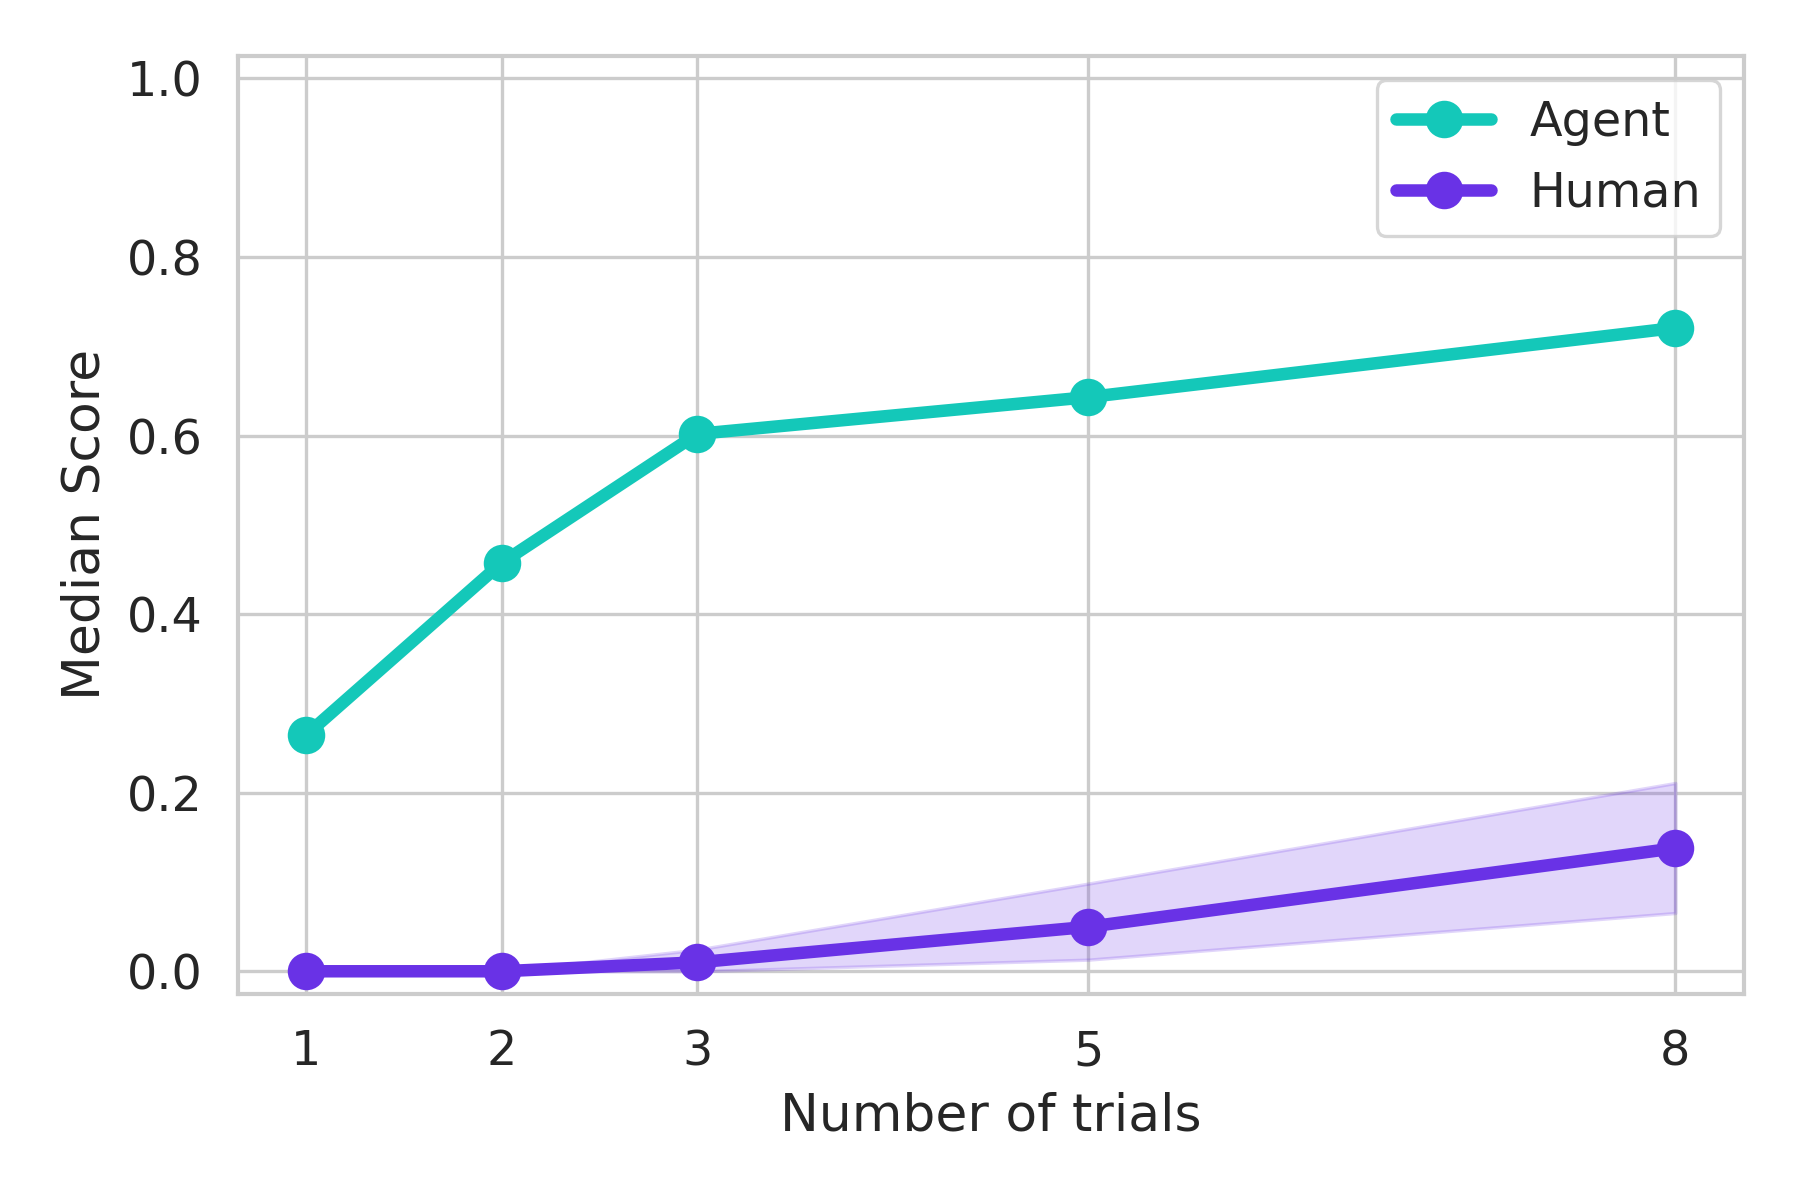
\includegraphics[width=\linewidth]{figures/human_scale_adaptation.png}
        \vskip -3pt \caption{}
        \label{fig:human_scale_adaptation}
    \end{subfigure}
    \begin{subfigure}[b]{0.47\textwidth}
        \centering
        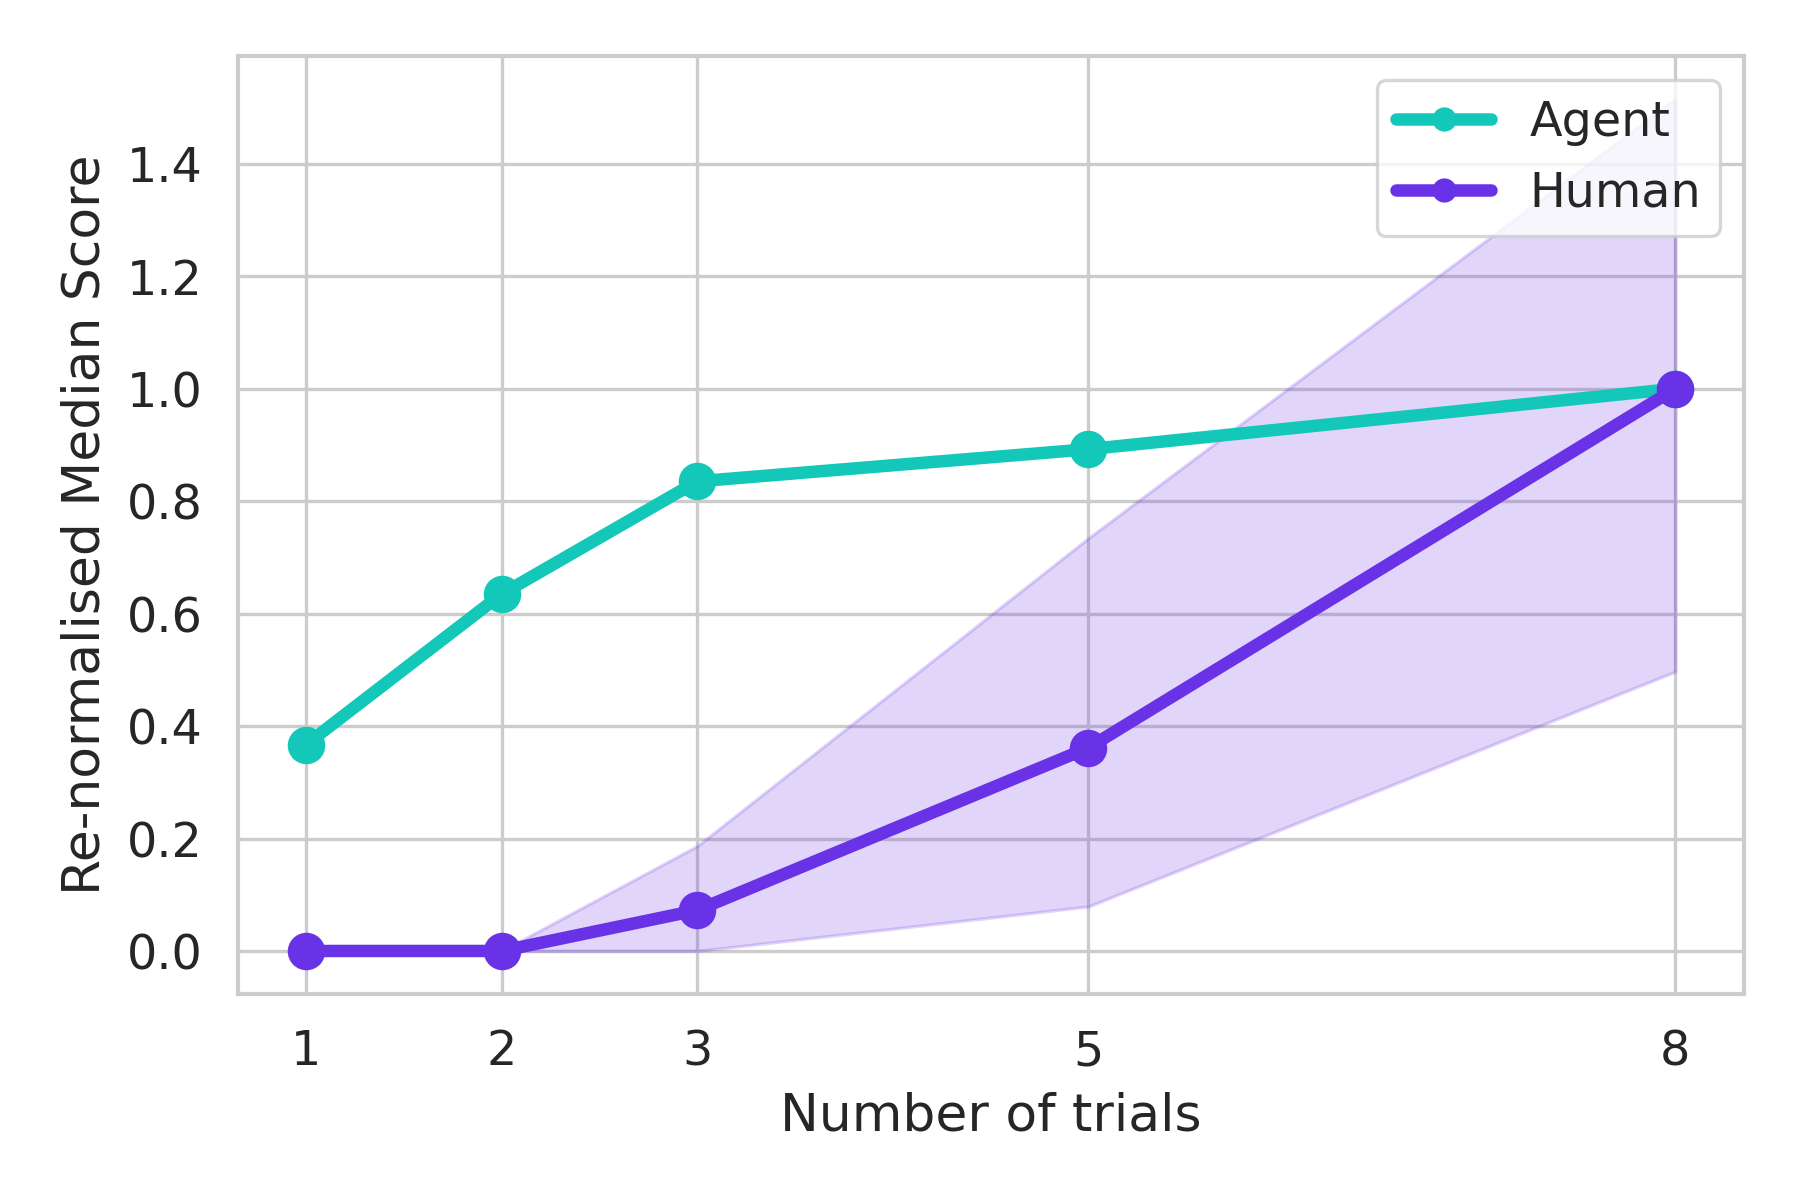
\includegraphics[width=\linewidth]{figures/human_scale_adaptation_renorm.png}
        \vskip -3pt \caption{}
        \label{fig:human_scale_adaptation_renorm}
    \end{subfigure}

    \caption{\textbf{Human-timescale adaptation.} We report median normalised last-trial score across 30 hand-authored tasks as a function of number of trials for AdA and human players. Both AdA and the human players improve their performance with increasing number of trials, indicating that AdA is capable of human-timescale adaptation. \textbf{(a)} shows the results using our standard per-task normalisation scheme. \textbf{(b)} re-normalises the results by the maximum score per player-type to account for systematic differences between the agent and human players. In particular, human players reported lag while playing which may have resulted in lower scores.}
\end{figure}

\begin{figure}[htb]
    \centering
    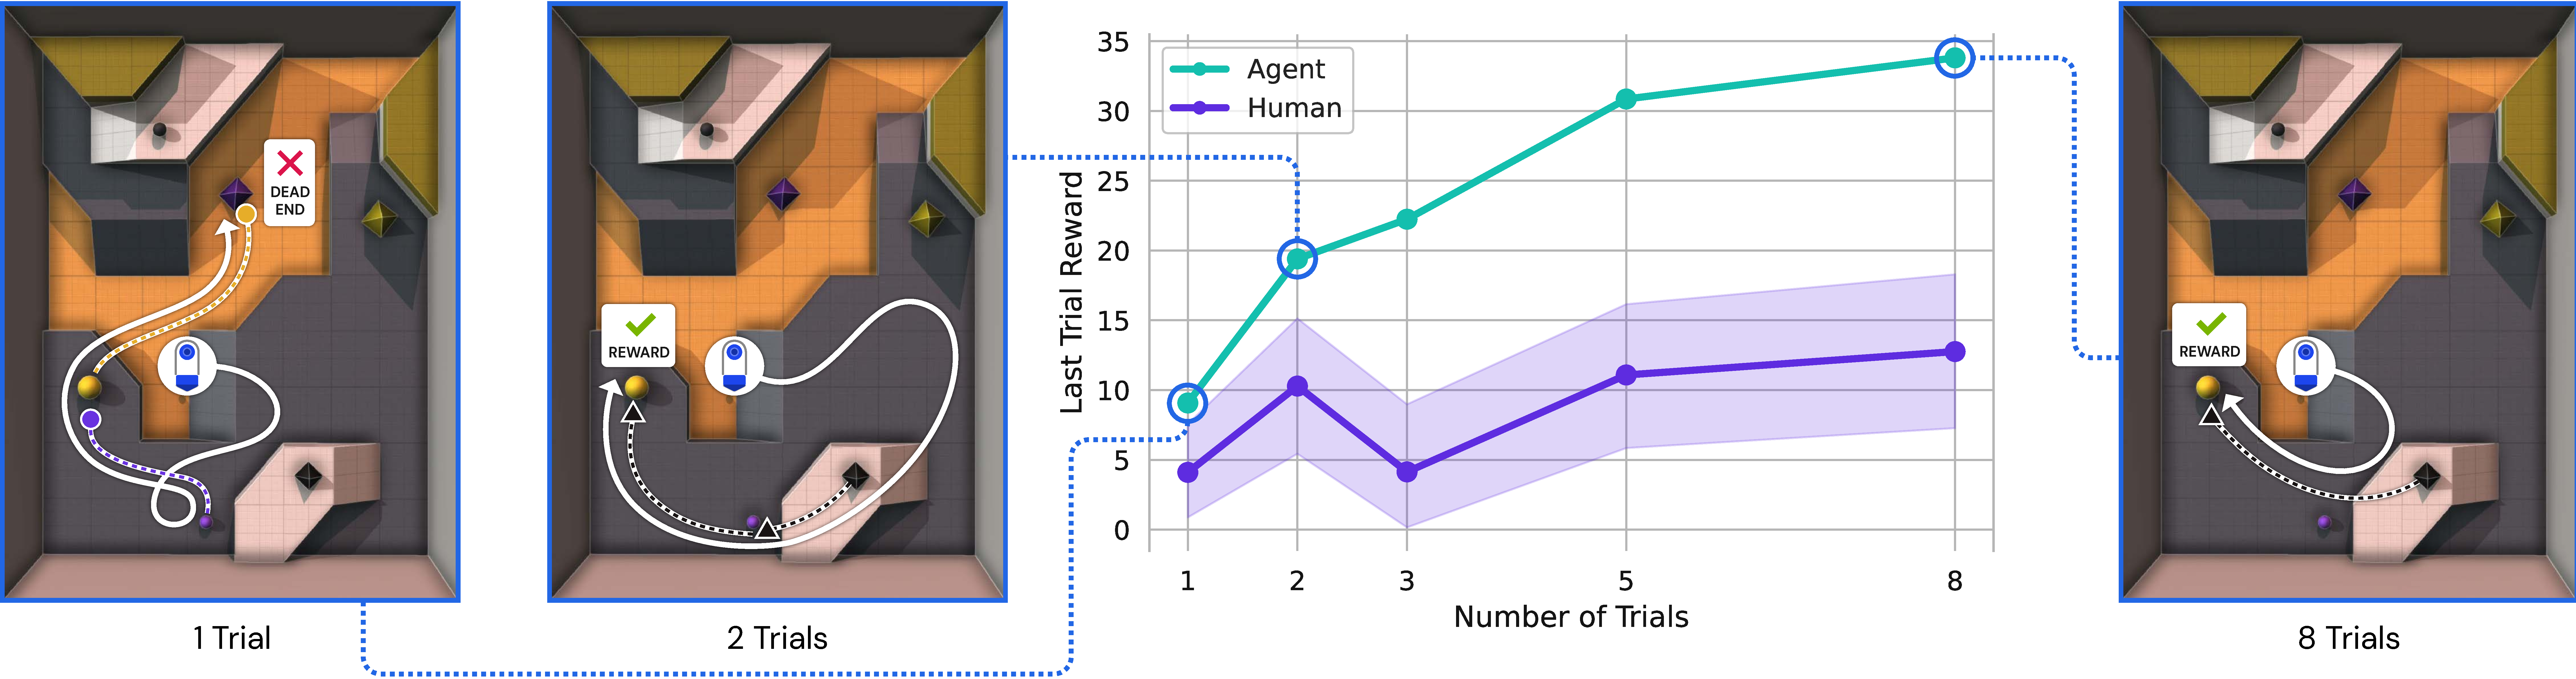
\includegraphics[width=1.0\linewidth]{figures/tasks/trajectories/trajectories_wrong_pair_disappears.pdf}
    \caption{\textbf{Experimentation, success and refinement.} We report average performance and representative behaviour of AdA on the probe task \texttt{Wrong Pair Disappears} when evaluated with various numbers of trials. AdA's performance increases when given more trials, showing test-time adaptation. The top-down view images show representative last-trial trajectories when given different numbers of total trials. A corresponding \href{https://youtu.be/FCDLu4iTBGE}{video} for the case $k = 3$ shows the behaviour across all trials within one episode.}
    \label{fig:probe_task_performance}
\end{figure}

We compare the performance of AdA to that of a set of human players on $30$ held-out hand-authored probe tasks, seeking to assess whether AdA adapts on the same timescale as humans. Figure \ref{fig:human_scale_adaptation} shows the median scores for AdA and for human players as a function of number of trials. Both AdA and human players were able to improve their score as they experienced more trials of the tasks, indicating that AdA exhibits human-timescale adaptation on this set of probe tasks. We provide more details of the scores obtained on each task in Figure \ref{fig:human_scale_adaptation_all_tasks}. This reveals a small set of tasks which humans can solve but AdA can't, such as the \texttt{Spacer Tool} task: in this task one object must be used as a tool to move another, a situation which is extremely rare in XLand. There are also tasks like \texttt{Small Workstation, All Rules Visible} which can be solved by AdA but not by humans, likely due to complex control requirements. The majority of tasks, however, show adaptation from both humans and AdA, with the slopes of AdA's score being as steep as, if not steeper than, those of the human players, especially for lower numbers of trials. For full details of our human experiment design, see Appendix \ref{app:human-data-collection}.

Figure~\ref{fig:probe_task_performance} analyses the behaviour of AdA in more detail on a specific held-out task. The increase in score with a larger number of trials indicates that the task is solved more consistently and more quickly when given a larger number of trials. Examining the trajectories for different numbers of trials, we can explain this effect in terms of the behaviour of AdA. When given $1$ or $2$ trials AdA's behaviour shows structured hypothesis-driven exploration: trying out different combinations of objects and coming across the solution or a dead end. Once the solution is found, AdA refines its strategy on subsequent trials, gathering the correct objects with more efficiency and combining them in the right way. Thus AdA is able to generate a higher last-trial score when provided with more trials for refinement. When given $8$ trials, the last-trial performance is close to that of the fine-tuned agent. We observe this pattern of behaviour consistently across many of our held-out probe tasks; see videos on our \href{http://sites.google.com/view/adaptive-agent/}{microsite}.

\paragraph{Multi-agent.} We train a separate agent on a mixture of fully-cooperative multi-agent and single-agent tasks to explore adaptation in the multi-agent setting. In fully-cooperative multi-agent tasks, both players have the same goal. Such tasks typically have multiple Nash equilibria \citep{DBLP:journals/corr/abs-2012-08630}. When faced with a new problem, agents must adapt on-the-fly to agree on a single equilibrium of maximal mutual benefit \citep{stone2010ad, hu2020other, https://doi.org/10.48550/arxiv.2209.14344}. This gives rise to a variety of interesting strategic novelties that are absent in the purely single-agent setting, including emergent division-of-labour and physical coordination. Both of these behaviours have received extensive study in the multi-agent RL literature (e.g. \cite{wang2020roma, https://doi.org/10.48550/arxiv.2006.06051, strouse2021collaborating, gronauer2022multi}); here for the first time to our knowledge, we demonstrate that these behaviours can emerge at test time in few-shot on held-out tasks. Co-players for our training tasks are generated using fictitious self-play \citep{heinrich2015fictitious} and then curated using PLR, as in \citet{samvelyan2022maestro}. For more details, see Table \ref{tab:human-timescale-settings} and Appendix~\ref{app:multi_agent_training}.

\begin{figure}[t!]
    \centering
    \begin{subfigure}[b]{0.48\textwidth}
        \centering
        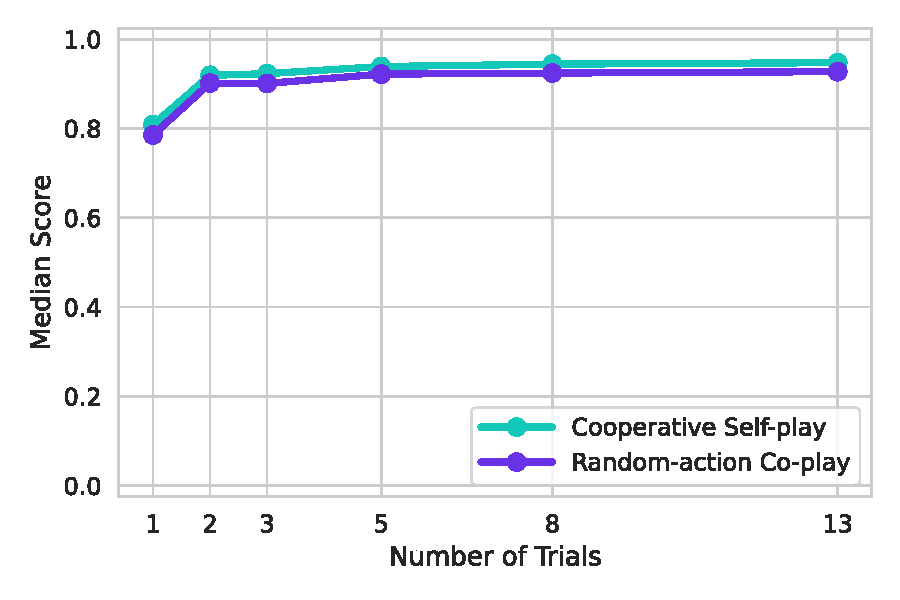
\includegraphics[width=\linewidth]{figures/self-play_vs_single-agent_perc50.pdf}
        \vskip -3pt \caption{}
    \end{subfigure}
    \begin{subfigure}[b]{0.48\textwidth}
        \centering
        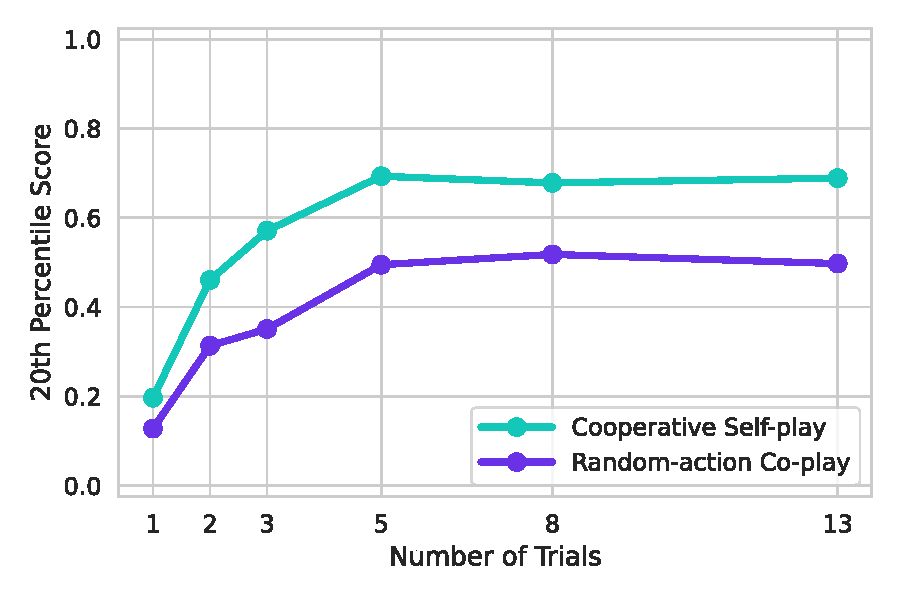
\includegraphics[width=\linewidth]{figures/self-play_vs_single-agent_perc20.pdf}
        \vskip -3pt \caption{}
    \end{subfigure}
    \caption{
        \textbf{Two heads are better than one.} Cooperative self-play outperforms single-agent performance on the test set of two-player cooperative held-out tasks. For this evaluation we restrict ourselves to tasks whose goals and production rules do not refer to players and which are solvable by a single player (216/1000 test tasks). To produce the purple curve, we evaluate AdA twice per task when playing with a random-action policy co-player, once playing as the first and once as the second player, and take the maximum score over both evaluations before cross-task aggregation. This accounts for possible advantages playing as one player might have over playing as the other in a task.
        \textbf{(a)} Median score.
        \textbf{(b)} 20\textsuperscript{th} percentile score.
    }
\label{fig:self_play_vs_single_agent}
\end{figure}

\begin{figure}[t!]
    \centering
    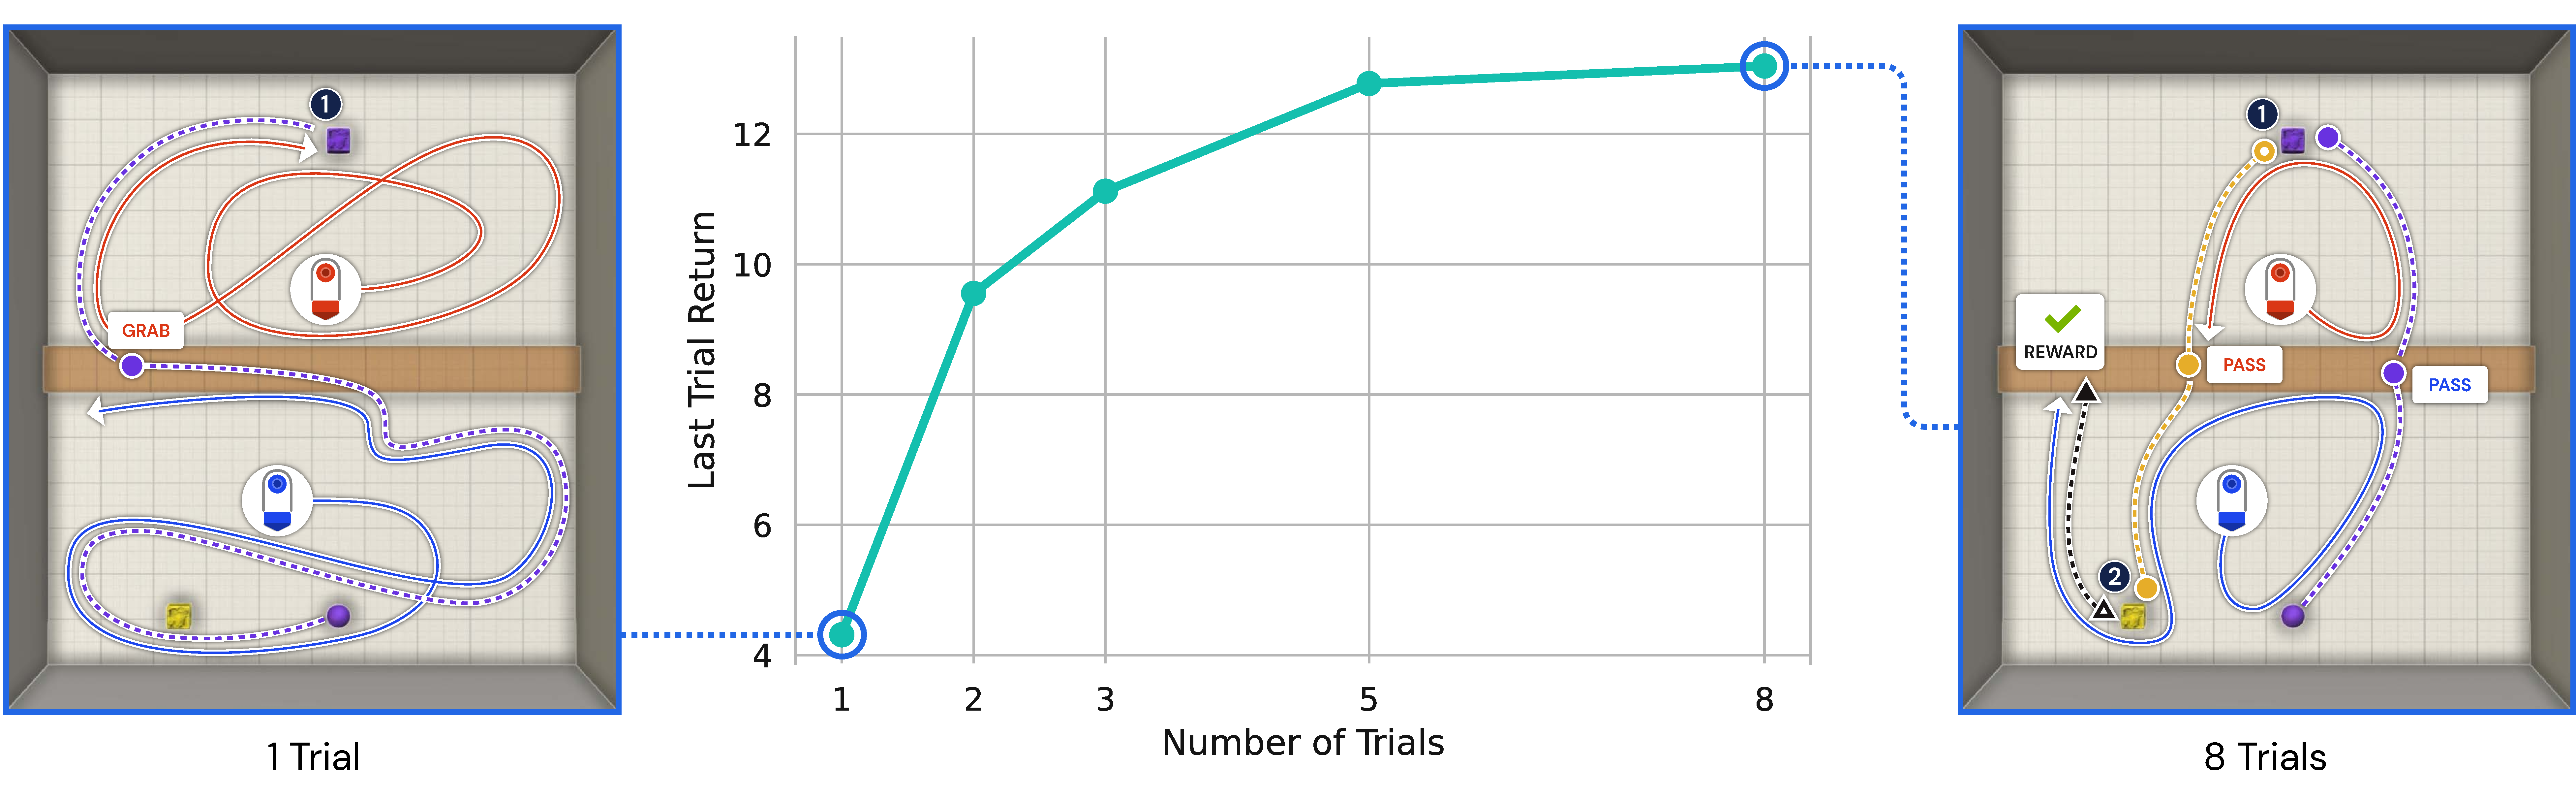
\includegraphics[width=1.0\linewidth]{figures/tasks/trajectories/trajectories_pass_over_wall_repeatedly.pdf}
    \caption{\textbf{Multi-agent coordination.} We report average performance and representative behaviour of AdA on the probe task \texttt{Pass Over the Wall Repeatedly} when evaluated in self-play with various numbers of trials. AdA's performance increases when given more trials, showing test-time adaptation. The top-down view images show representative last-trial trajectories when given different numbers of total trials. A corresponding \href{https://youtu.be/Rnz2MFgeicc}{video} for the case $k = 5$ shows the behaviour across all trials within one episode.}
    \label{fig:multi_agent_probe_forced_coop}
\end{figure}

Analogously with the single-agent setting, we find strong evidence of adaptation across almost $90 \%$ of the space of held-out test tasks (Figure \ref{fig:multi_agent_percentiles}). Futhermore, we evaluate the resulting agent on a held-out test set of cooperative multi-agent tasks in two ways: in self-play and in co-play with a random-action policy. As shown in Figure~\ref{fig:self_play_vs_single_agent}, self-play outperforms co-play with a random-action policy by a large margin both in a zero-shot and in a few-shot setting. This indicates that the agents are dividing the labour required to solve the tasks, thereby solving the task more quickly (or at all) and improving their shared performance.

Examples of emergent social behaviour in self-play are shown in Figures~\ref{fig:multi_agent_probe_forced_coop} and \ref{fig:multi_agent_probe_emergent_coop}. When given only a few trials, the agents explore the space of possible solutions, sometimes operating independently and sometimes together. Given more trials, once the agents find a solution, they optimise their paths by coordinating physically and dividing labour to solve the task efficiently. This behaviour emerges from adaptation at test time and was not explicitly incentivised during training, other than through the high-level fully cooperative reward function. Videos of such behavior in a variety of tasks are available on our \href{http://sites.google.com/view/adaptive-agent/}{microsite}.
